\section{Additional Results}
\label{sec:appendix-results}

This appendix reports the complete numerical results underlying the paper's
plots. The guide below follows the order of the corresponding main-text
analyses and points to the relevant figures and tables. In matched-budget
method comparisons, boldface marks the best displayed value and underlining
marks the second-best; table panel headings state the metric direction.

\subsection{Guide to the Complete Results}
\label{sec:appendix-guide}

\paragraph{Headline method comparison.}
The exact values behind the principal accuracy--efficiency
comparison is in Table~\ref{tab:main-fixed-budget-complete}; it reports
executed questions, execution fraction, pass-rate MAE, Spearman correlation,
and Kendall's $\tau$ for every method and operating point in
Figures~\ref{fig:main-mae} and~\ref{fig:main-ranking}.
Table~\ref{tab:cache-complete} gives the
corresponding threshold-level results for historical caching. Together, these
tables provide the complete numerical record for the two headline plots.

\paragraph{Fixed-subset design results.}
Figures~\ref{fig:fixed-subset-spearman} and
\ref{fig:fixed-subset-kendall} give the full ranking-fidelity curves for the
selection-by-estimation comparison whose MAE results appear in
Figure~\ref{fig:fixed-subset-mae}. Table~\ref{tab:fixed-design-complete}
then collects all three metrics for every selector, estimator, and budget. 
% Use
% the figures to compare trends and the table to recover exact matched-budget
% values.

\paragraph{Adaptive-model design results.}
Figure~\ref{fig:adaptive-model-ranking} supplies the Spearman and Kendall views
corresponding to the MAE comparison in Figure~\ref{fig:adaptive-model-mae}.
Table~\ref{tab:adaptive-model-complete} reports the exact MAE and rank correlations
for Rasch adaptive testing, multidimensional 2PL adaptive testing, and random
sampling at every evaluated budget.

\paragraph{Cross-agent transfer results.}
Table~\ref{tab:cross-agent-run-counts} first defines the five held-out
families and their run counts. For the aggregate transfer result,
Figure~\ref{fig:cross-agent-transfer-ranking} and
Table~\ref{tab:transfer-pooled-complete} provide the pooled ranking curves
and all exact pooled metrics. 
Figures~\ref{fig:cross-agent-family-mae}--
\ref{fig:cross-agent-family-kendall} and
Tables~\ref{tab:transfer-family-a-complete}--
\ref{tab:transfer-family-e-complete} report the same results
separately for each agent family.

\paragraph{Calibration-window sensitivity.}
Figure~\ref{fig:calibration-window-ranking} gives the Spearman and Kendall
sensitivity curves that complement the MAE results in
Figure~\ref{fig:calibration-window-mae}. Table~\ref{tab:calibration-window-complete}
reports every window's start day, number of calibration runs, subset size, and
three fidelity metrics. 

\clearpage

\makeatletter
\setlength{\@fptop}{0pt}
\setlength{\@dblfptop}{0pt}
\makeatother

\begin{table*}[t]
  \centering
  \small
  \setlength{\tabcolsep}{3.5pt}
  \begin{tabular}{rrrrrr}
    \toprule
    \multicolumn{6}{l}{\textit{(a) Pass-rate MAE (percentage points; lower is better)}} \\
    $k$ & Exec. (\%) & Random & \shortstack{Difficulty\\weighted} & \shortstack{Difficulty\\gp-IRT} & \shortstack{Rasch\\adaptive} \\
    \midrule
    10 & 1.9 & 10.48 & \underline{8.10} & \textbf{7.57} & 10.94 \\
    20 & 3.9 & 7.22 & \underline{6.37} & \textbf{5.51} & 9.79 \\
    30 & 5.8 & 5.86 & \underline{4.63} & \textbf{4.35} & 6.50 \\
    50 & 9.6 & 4.41 & \underline{3.37} & \textbf{3.28} & 6.46 \\
    75 & 14.5 & 3.49 & \textbf{3.04} & \underline{3.05} & 3.51 \\
    100 & 19.3 & 2.94 & \underline{2.71} & \textbf{2.65} & 2.92 \\
    150 & 28.9 & 2.25 & \underline{2.01} & \textbf{2.00} & 2.07 \\
    200 & 38.5 & 1.79 & 1.43 & \underline{1.40} & \textbf{1.37} \\
    250 & 48.2 & 1.46 & 1.17 & \underline{1.15} & \textbf{1.03} \\
    300 & 57.8 & 1.18 & 1.06 & \underline{0.99} & \textbf{0.79} \\
    350 & 67.4 & 0.93 & 0.77 & \underline{0.73} & \textbf{0.60} \\
    400 & 77.1 & 0.69 & 0.51 & \underline{0.47} & \textbf{0.42} \\
    \midrule
    \multicolumn{6}{l}{\textit{(b) Spearman correlation (higher is better)}} \\
    $k$ & Exec. (\%) & Random & \shortstack{Difficulty\\weighted} & \shortstack{Difficulty\\gp-IRT} & \shortstack{Rasch\\adaptive} \\
    \midrule
    10 & 1.9 & 0.559 & \underline{0.586} & \textbf{0.598} & 0.446 \\
    20 & 3.9 & 0.692 & \textbf{0.804} & \underline{0.803} & 0.510 \\
    30 & 5.8 & 0.757 & \textbf{0.803} & \underline{0.796} & 0.667 \\
    50 & 9.6 & 0.835 & \underline{0.876} & \textbf{0.883} & 0.697 \\
    75 & 14.5 & \underline{0.884} & \textbf{0.924} & \textbf{0.924} & 0.883 \\
    100 & 19.3 & 0.911 & \textbf{0.930} & \textbf{0.930} & \underline{0.923} \\
    150 & 28.9 & 0.941 & \underline{0.960} & \textbf{0.961} & 0.948 \\
    200 & 38.5 & \underline{0.957} & \textbf{0.972} & \textbf{0.972} & \textbf{0.972} \\
    250 & 48.2 & 0.967 & 0.977 & \underline{0.978} & \textbf{0.979} \\
    300 & 57.8 & 0.975 & 0.980 & \underline{0.981} & \textbf{0.986} \\
    350 & 67.4 & 0.983 & 0.987 & \underline{0.988} & \textbf{0.992} \\
    400 & 77.1 & 0.989 & 0.993 & \underline{0.994} & \textbf{0.995} \\
    \midrule
    \multicolumn{6}{l}{\textit{(c) Kendall's Tau (higher is better)}} \\
    $k$ & Exec. (\%) & Random & \shortstack{Difficulty\\weighted} & \shortstack{Difficulty\\gp-IRT} & \shortstack{Rasch\\adaptive} \\
    \midrule
    10 & 1.9 & 0.426 & \textbf{0.434} & \underline{0.431} & 0.323 \\
    20 & 3.9 & 0.531 & \textbf{0.632} & \underline{0.619} & 0.383 \\
    30 & 5.8 & 0.585 & \textbf{0.617} & \underline{0.607} & 0.517 \\
    50 & 9.6 & 0.661 & \underline{0.692} & \textbf{0.700} & 0.570 \\
    75 & 14.5 & 0.715 & \textbf{0.764} & \textbf{0.764} & \underline{0.719} \\
    100 & 19.3 & 0.751 & \textbf{0.771} & \underline{0.770} & 0.760 \\
    150 & 28.9 & 0.798 & \underline{0.832} & \textbf{0.834} & 0.813 \\
    200 & 38.5 & 0.829 & 0.857 & \underline{0.859} & \textbf{0.873} \\
    250 & 48.2 & 0.853 & \underline{0.874} & \underline{0.874} & \textbf{0.900} \\
    300 & 57.8 & 0.875 & 0.884 & \underline{0.887} & \textbf{0.920} \\
    350 & 67.4 & 0.898 & 0.912 & \underline{0.915} & \textbf{0.944} \\
    400 & 77.1 & 0.923 & 0.937 & \underline{0.941} & \textbf{0.962} \\
    \bottomrule
  \end{tabular}
  \caption{Complete fixed-budget headline results on 287 held-out runs. Within each budget and metric, bold marks the best displayed value and underlining marks the second-best; emphasis is descriptive and does not denote statistical significance.}
  \label{tab:main-fixed-budget-complete}
\end{table*}


\FloatBarrier

\begin{table}[t]
  \centering
  \scriptsize
  \setlength{\tabcolsep}{2.2pt}
  \begin{tabular}{rrrrr}
    \toprule
    Threshold $q$ & Exec. (\%) & MAE (pp) & Spearman & Kendall \\
    \midrule
    0.30 & 20.3 & 7.36 & 0.904 & 0.732 \\
    0.29 & 21.4 & 7.19 & 0.913 & 0.747 \\
    0.28 & 22.4 & 7.06 & 0.918 & 0.755 \\
    0.27 & 23.7 & 6.86 & 0.922 & 0.760 \\
    0.26 & 25.0 & 6.67 & 0.925 & 0.766 \\
    0.25 & 26.2 & 6.47 & 0.932 & 0.780 \\
    0.24 & 27.5 & 6.22 & 0.933 & 0.781 \\
    0.23 & 29.1 & 5.97 & 0.938 & 0.790 \\
    0.22 & 30.5 & 5.78 & 0.942 & 0.798 \\
    0.21 & 32.2 & 5.54 & 0.948 & 0.809 \\
    0.20 & 33.6 & 5.32 & 0.953 & 0.820 \\
    0.19 & 35.5 & 5.05 & 0.957 & 0.831 \\
    0.18 & 37.0 & 4.84 & 0.961 & 0.840 \\
    0.17 & 38.7 & 4.62 & 0.963 & 0.846 \\
    0.16 & 40.1 & 4.44 & 0.967 & 0.855 \\
    0.15 & 41.9 & 4.20 & 0.969 & 0.862 \\
    0.14 & 43.7 & 4.01 & 0.972 & 0.869 \\
    0.13 & 45.6 & 3.77 & 0.974 & 0.876 \\
    0.12 & 47.2 & 3.61 & 0.977 & 0.884 \\
    0.11 & 48.9 & 3.42 & 0.979 & 0.890 \\
    0.10 & 50.7 & 3.22 & 0.981 & 0.899 \\
    0.09 & 52.9 & 2.97 & 0.982 & 0.905 \\
    0.08 & 55.1 & 2.74 & 0.983 & 0.911 \\
    0.07 & 57.6 & 2.48 & 0.984 & 0.915 \\
    0.06 & 59.7 & 2.27 & 0.985 & 0.920 \\
    0.05 & 62.4 & 2.04 & 0.986 & 0.923 \\
    0.04 & 65.4 & 1.80 & 0.989 & 0.935 \\
    0.03 & 69.1 & 1.54 & 0.992 & 0.943 \\
    0.02 & 73.5 & 1.23 & 0.995 & 0.957 \\
    0.01 & 79.0 & 0.91 & 0.996 & 0.967 \\
    0.00 & 81.6 & 0.81 & 0.997 & 0.974 \\
    \bottomrule
  \end{tabular}
  \caption{Complete historical-caching threshold sweep on 287 held-out runs. Rows are ordered by mean execution fraction. MAE is in percentage points.}
  \label{tab:cache-complete}
\end{table}


\FloatBarrier

\begin{figure*}[t]
    \centering
    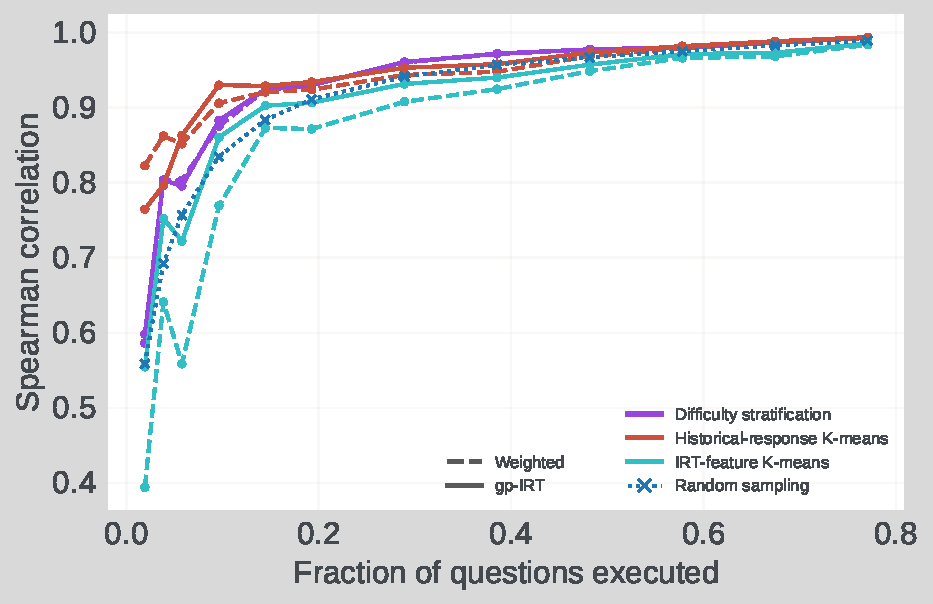
\includegraphics[width=0.82\textwidth]{figures/fixed_subset_spearman.pdf}
    \caption{Spearman ranking fidelity for the fixed-subset
    selection-by-estimation comparison. Higher values are better. All methods
    use the same 287 held-out evaluation runs and the same question budgets;
    random sampling is averaged over 20 seeds.}
    \label{fig:fixed-subset-spearman}
\end{figure*}

\begin{figure*}[t]
    \centering
    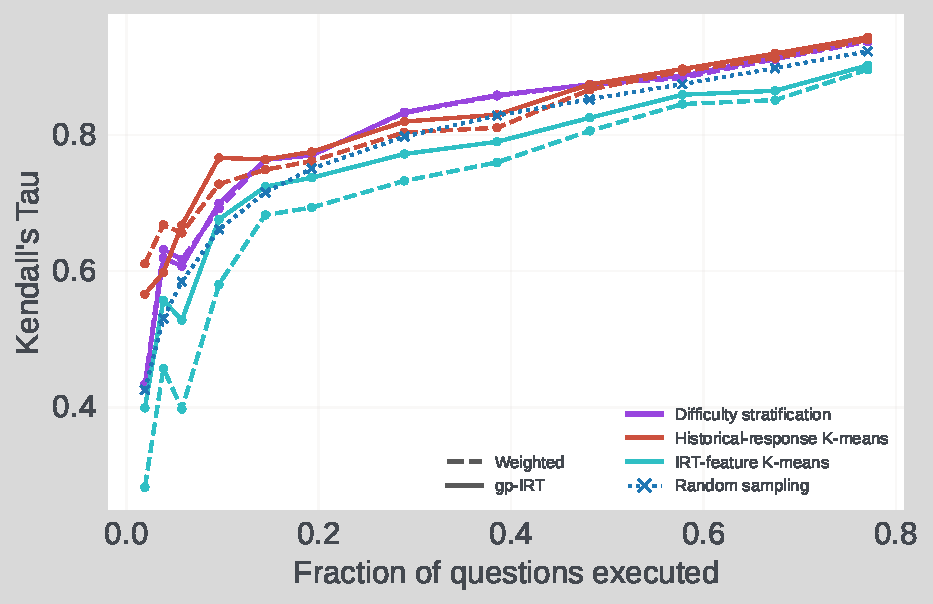
\includegraphics[width=0.82\textwidth]{figures/fixed_subset_kendall.pdf}
    \caption{Kendall's $\tau$ ranking fidelity for the fixed-subset
    selection-by-estimation comparison. Higher values are better. The test
    population, budgets, and random-sampling seeds match
    Figure~\ref{fig:fixed-subset-spearman}.}
    \label{fig:fixed-subset-kendall}
\end{figure*}

\FloatBarrier

\begin{table*}[t]
  \centering
  \scriptsize
  \setlength{\tabcolsep}{2.4pt}
  \begin{tabular}{rrrrrrrrr}
    \toprule
    \multicolumn{9}{l}{\textit{(a) Pass-rate MAE (percentage points; lower is better)}} \\
    $k$ & Exec. (\%) & Random & \shortstack{Difficulty\\weighted} & \shortstack{Difficulty\\gp-IRT} & \shortstack{Hist. K-means\\weighted} & \shortstack{Hist. K-means\\gp-IRT} & \shortstack{IRT K-means\\weighted} & \shortstack{IRT K-means\\gp-IRT} \\
    \midrule
    10 & 1.9 & 10.48 & 8.10 & 7.57 & \textbf{6.24} & 10.11 & 10.44 & \underline{6.53} \\
    20 & 3.9 & 7.22 & 6.37 & 5.51 & \textbf{4.51} & 5.82 & 8.00 & \underline{5.00} \\
    30 & 5.8 & 5.86 & 4.63 & \underline{4.35} & 4.37 & \textbf{3.88} & 9.10 & 5.27 \\
    50 & 9.6 & 4.41 & 3.37 & \underline{3.28} & 3.44 & \textbf{2.77} & 7.95 & 5.47 \\
    75 & 14.5 & 3.49 & \underline{3.04} & 3.05 & 4.12 & \textbf{2.96} & 4.76 & 3.29 \\
    100 & 19.3 & 2.94 & 2.71 & \underline{2.65} & 2.93 & \textbf{2.46} & 4.21 & 2.88 \\
    150 & 28.9 & 2.25 & \underline{2.01} & \textbf{2.00} & 2.61 & 2.13 & 3.36 & 2.71 \\
    200 & 38.5 & 1.79 & \underline{1.43} & \textbf{1.40} & 2.51 & 2.12 & 2.47 & 2.07 \\
    250 & 48.2 & 1.46 & \underline{1.17} & \textbf{1.15} & 1.75 & 1.56 & 2.06 & 1.70 \\
    300 & 57.8 & 1.18 & \underline{1.06} & \textbf{0.99} & 1.38 & 1.27 & 1.63 & 1.50 \\
    350 & 67.4 & 0.93 & \underline{0.77} & \textbf{0.73} & 1.18 & 1.05 & 1.52 & 1.42 \\
    400 & 77.1 & 0.69 & \underline{0.51} & \textbf{0.47} & 1.07 & 0.93 & 0.94 & 0.88 \\
    \midrule
    \multicolumn{9}{l}{\textit{(b) Spearman correlation (higher is better)}} \\
    $k$ & Exec. (\%) & Random & \shortstack{Difficulty\\weighted} & \shortstack{Difficulty\\gp-IRT} & \shortstack{Hist. K-means\\weighted} & \shortstack{Hist. K-means\\gp-IRT} & \shortstack{IRT K-means\\weighted} & \shortstack{IRT K-means\\gp-IRT} \\
    \midrule
    10 & 1.9 & 0.559 & 0.586 & 0.598 & \textbf{0.823} & \underline{0.765} & 0.394 & 0.555 \\
    20 & 3.9 & 0.692 & \underline{0.804} & 0.803 & \textbf{0.862} & 0.796 & 0.641 & 0.752 \\
    30 & 5.8 & 0.757 & 0.803 & 0.796 & \underline{0.852} & \textbf{0.863} & 0.559 & 0.722 \\
    50 & 9.6 & 0.835 & 0.876 & 0.883 & \underline{0.906} & \textbf{0.930} & 0.769 & 0.861 \\
    75 & 14.5 & 0.884 & \underline{0.924} & \underline{0.924} & 0.921 & \textbf{0.929} & 0.873 & 0.903 \\
    100 & 19.3 & 0.911 & \underline{0.930} & \underline{0.930} & 0.924 & \textbf{0.934} & 0.872 & 0.907 \\
    150 & 28.9 & 0.941 & \underline{0.960} & \textbf{0.961} & 0.944 & 0.953 & 0.908 & 0.932 \\
    200 & 38.5 & 0.957 & \textbf{0.972} & \textbf{0.972} & 0.948 & \underline{0.958} & 0.925 & 0.940 \\
    250 & 48.2 & 0.967 & \underline{0.977} & \textbf{0.978} & 0.969 & 0.974 & 0.949 & 0.957 \\
    300 & 57.8 & 0.975 & 0.980 & \underline{0.981} & 0.979 & \textbf{0.982} & 0.966 & 0.971 \\
    350 & 67.4 & 0.983 & 0.987 & \underline{0.988} & 0.987 & \textbf{0.989} & 0.968 & 0.973 \\
    400 & 77.1 & 0.989 & \underline{0.993} & \textbf{0.994} & \underline{0.993} & \textbf{0.994} & 0.984 & 0.986 \\
    \midrule
    \multicolumn{9}{l}{\textit{(c) Kendall's Tau (higher is better)}} \\
    $k$ & Exec. (\%) & Random & \shortstack{Difficulty\\weighted} & \shortstack{Difficulty\\gp-IRT} & \shortstack{Hist. K-means\\weighted} & \shortstack{Hist. K-means\\gp-IRT} & \shortstack{IRT K-means\\weighted} & \shortstack{IRT K-means\\gp-IRT} \\
    \midrule
    10 & 1.9 & 0.426 & 0.434 & 0.431 & \textbf{0.611} & \underline{0.566} & 0.282 & 0.399 \\
    20 & 3.9 & 0.531 & \underline{0.632} & 0.619 & \textbf{0.668} & 0.598 & 0.457 & 0.557 \\
    30 & 5.8 & 0.585 & 0.617 & 0.607 & \underline{0.656} & \textbf{0.668} & 0.397 & 0.528 \\
    50 & 9.6 & 0.661 & 0.692 & 0.700 & \underline{0.728} & \textbf{0.766} & 0.580 & 0.676 \\
    75 & 14.5 & 0.715 & \textbf{0.764} & \textbf{0.764} & \underline{0.749} & \textbf{0.764} & 0.682 & 0.724 \\
    100 & 19.3 & 0.751 & \underline{0.771} & 0.770 & 0.762 & \textbf{0.775} & 0.693 & 0.737 \\
    150 & 28.9 & 0.798 & \underline{0.832} & \textbf{0.834} & 0.804 & 0.820 & 0.733 & 0.772 \\
    200 & 38.5 & 0.829 & \underline{0.857} & \textbf{0.859} & 0.811 & 0.830 & 0.760 & 0.790 \\
    250 & 48.2 & 0.853 & \textbf{0.874} & \textbf{0.874} & \underline{0.867} & \textbf{0.874} & 0.806 & 0.825 \\
    300 & 57.8 & 0.875 & 0.884 & 0.887 & \underline{0.893} & \textbf{0.897} & 0.846 & 0.859 \\
    350 & 67.4 & 0.898 & 0.912 & \underline{0.915} & 0.913 & \textbf{0.920} & 0.851 & 0.865 \\
    400 & 77.1 & 0.923 & 0.937 & \underline{0.941} & 0.940 & \textbf{0.944} & 0.896 & 0.902 \\
    \bottomrule
  \end{tabular}
  \caption{Complete fixed-subset selection and estimation results on 287 held-out runs. Bold and underlining mark the best and second-best displayed values at each budget, respectively.}
  \label{tab:fixed-design-complete}
\end{table*}


\FloatBarrier

\begin{figure*}[t]
    \centering
    \begin{subfigure}[t]{0.49\textwidth}
        \centering
        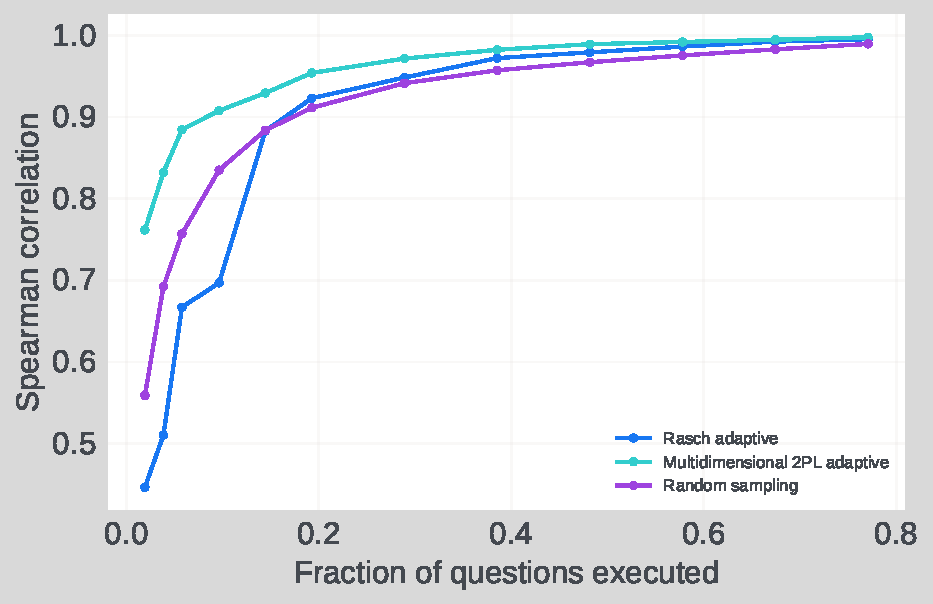
\includegraphics[width=\linewidth]{figures/adaptive_model_spearman.pdf}
        \caption{Spearman correlation.}
        \label{fig:adaptive-model-spearman}
    \end{subfigure}
    \hfill
    \begin{subfigure}[t]{0.49\textwidth}
        \centering
        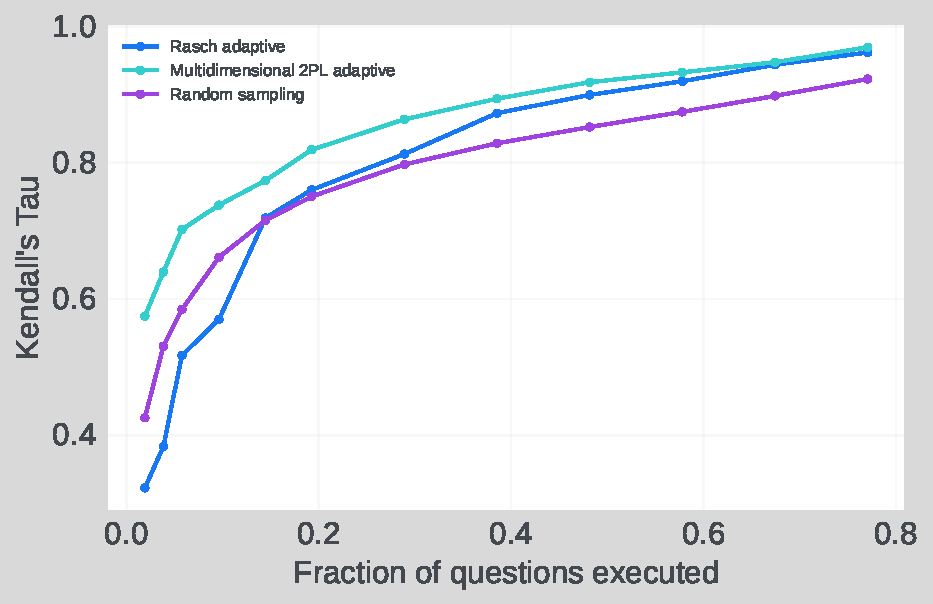
\includegraphics[width=\linewidth]{figures/adaptive_model_kendall.pdf}
        \caption{Kendall's $\tau$.}
        \label{fig:adaptive-model-kendall}
    \end{subfigure}
    \caption{Ranking fidelity for the adaptive-model comparison. Higher values
    are better. Both panels use the same 287 held-out evaluation runs and
    question budgets as Figure~\ref{fig:adaptive-model-mae}; random sampling is
    averaged over 20 seeds.}
    \label{fig:adaptive-model-ranking}
\end{figure*}

\FloatBarrier

\begin{table*}[t]
  \centering
  \small
  \setlength{\tabcolsep}{3.5pt}
  \begin{tabular}{rrrrr}
    \toprule
    \multicolumn{5}{l}{\textit{(a) Pass-rate MAE (percentage points; lower is better)}} \\
    $k$ & Exec. (\%) & Random & \shortstack{Rasch\\adaptive} & \shortstack{Multidimensional 2PL\\adaptive} \\
    \midrule
    10 & 1.9 & \underline{10.48} & 10.94 & \textbf{5.07} \\
    20 & 3.9 & \underline{7.22} & 9.79 & \textbf{3.90} \\
    30 & 5.8 & \underline{5.86} & 6.50 & \textbf{3.27} \\
    50 & 9.6 & \underline{4.41} & 6.46 & \textbf{2.81} \\
    75 & 14.5 & \underline{3.49} & 3.51 & \textbf{2.39} \\
    100 & 19.3 & 2.94 & \underline{2.92} & \textbf{1.97} \\
    150 & 28.9 & 2.25 & \underline{2.07} & \textbf{1.44} \\
    200 & 38.5 & 1.79 & \underline{1.37} & \textbf{1.03} \\
    250 & 48.2 & 1.46 & \underline{1.03} & \textbf{0.73} \\
    300 & 57.8 & 1.18 & \underline{0.79} & \textbf{0.58} \\
    350 & 67.4 & 0.93 & \underline{0.60} & \textbf{0.46} \\
    400 & 77.1 & 0.69 & \underline{0.42} & \textbf{0.29} \\
    \midrule
    \multicolumn{5}{l}{\textit{(b) Spearman correlation (higher is better)}} \\
    $k$ & Exec. (\%) & Random & \shortstack{Rasch\\adaptive} & \shortstack{Multidimensional 2PL\\adaptive} \\
    \midrule
    10 & 1.9 & \underline{0.559} & 0.446 & \textbf{0.762} \\
    20 & 3.9 & \underline{0.692} & 0.510 & \textbf{0.832} \\
    30 & 5.8 & \underline{0.757} & 0.667 & \textbf{0.884} \\
    50 & 9.6 & \underline{0.835} & 0.697 & \textbf{0.908} \\
    75 & 14.5 & \underline{0.884} & 0.883 & \textbf{0.929} \\
    100 & 19.3 & 0.911 & \underline{0.923} & \textbf{0.954} \\
    150 & 28.9 & 0.941 & \underline{0.948} & \textbf{0.972} \\
    200 & 38.5 & 0.957 & \underline{0.972} & \textbf{0.982} \\
    250 & 48.2 & 0.967 & \underline{0.979} & \textbf{0.989} \\
    300 & 57.8 & 0.975 & \underline{0.986} & \textbf{0.992} \\
    350 & 67.4 & 0.983 & \underline{0.992} & \textbf{0.995} \\
    400 & 77.1 & 0.989 & \underline{0.995} & \textbf{0.998} \\
    \midrule
    \multicolumn{5}{l}{\textit{(c) Kendall's Tau (higher is better)}} \\
    $k$ & Exec. (\%) & Random & \shortstack{Rasch\\adaptive} & \shortstack{Multidimensional 2PL\\adaptive} \\
    \midrule
    10 & 1.9 & \underline{0.426} & 0.323 & \textbf{0.575} \\
    20 & 3.9 & \underline{0.531} & 0.383 & \textbf{0.640} \\
    30 & 5.8 & \underline{0.585} & 0.517 & \textbf{0.702} \\
    50 & 9.6 & \underline{0.661} & 0.570 & \textbf{0.738} \\
    75 & 14.5 & 0.715 & \underline{0.719} & \textbf{0.774} \\
    100 & 19.3 & 0.751 & \underline{0.760} & \textbf{0.819} \\
    150 & 28.9 & 0.798 & \underline{0.813} & \textbf{0.864} \\
    200 & 38.5 & 0.829 & \underline{0.873} & \textbf{0.894} \\
    250 & 48.2 & 0.853 & \underline{0.900} & \textbf{0.918} \\
    300 & 57.8 & 0.875 & \underline{0.920} & \textbf{0.933} \\
    350 & 67.4 & 0.898 & \underline{0.944} & \textbf{0.948} \\
    400 & 77.1 & 0.923 & \underline{0.962} & \textbf{0.970} \\
    \bottomrule
  \end{tabular}
  \caption{Complete adaptive-model comparison on 287 held-out runs. Bold and underlining mark the best and second-best displayed values at each budget, respectively.}
  \label{tab:adaptive-model-complete}
\end{table*}


\FloatBarrier

\begin{table}[t]
  \centering
  \small
  \begin{tabular}{lr}
    \toprule
    Agent family & Evaluation runs \\
    \midrule
    Family A & 51 \\
    Family B & 146 \\
    Family C & 56 \\
    Family D & 34 \\
    Family E & 12 \\
    \midrule
    Total & 299 \\
    \bottomrule
  \end{tabular}
  \caption{Breakdown of transferred evaluation runs by anonymized agent family. The labels match the family-level figures and tables.}
  \label{tab:cross-agent-run-counts}
\end{table}


\FloatBarrier

\begin{figure*}[t]
    \centering
    \begin{subfigure}[t]{0.49\textwidth}
        \centering
        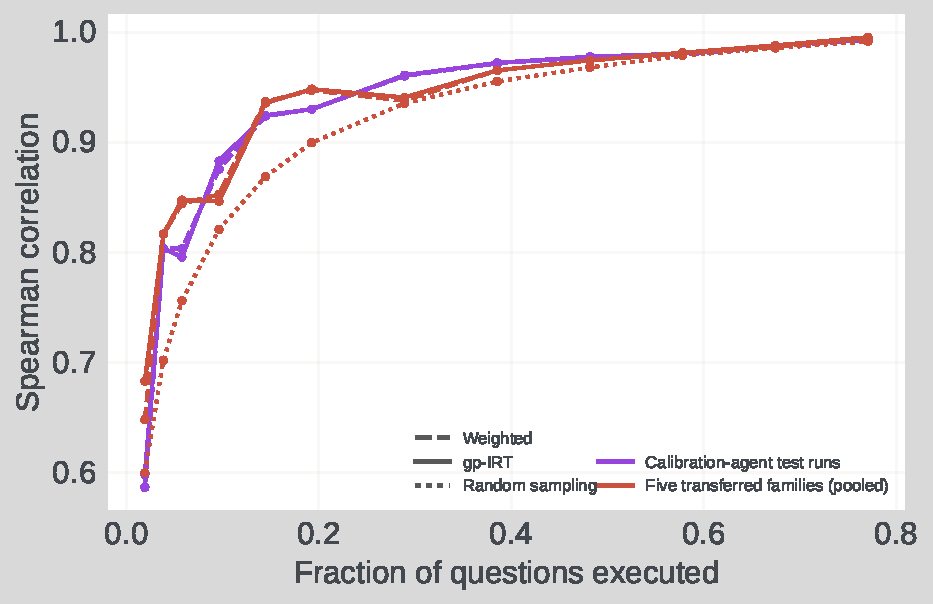
\includegraphics[width=\linewidth]{figures/cross_agent_transfer_spearman.pdf}
        \caption{Spearman correlation.}
        \label{fig:cross-agent-transfer-spearman}
    \end{subfigure}
    \hfill
    \begin{subfigure}[t]{0.49\textwidth}
        \centering
        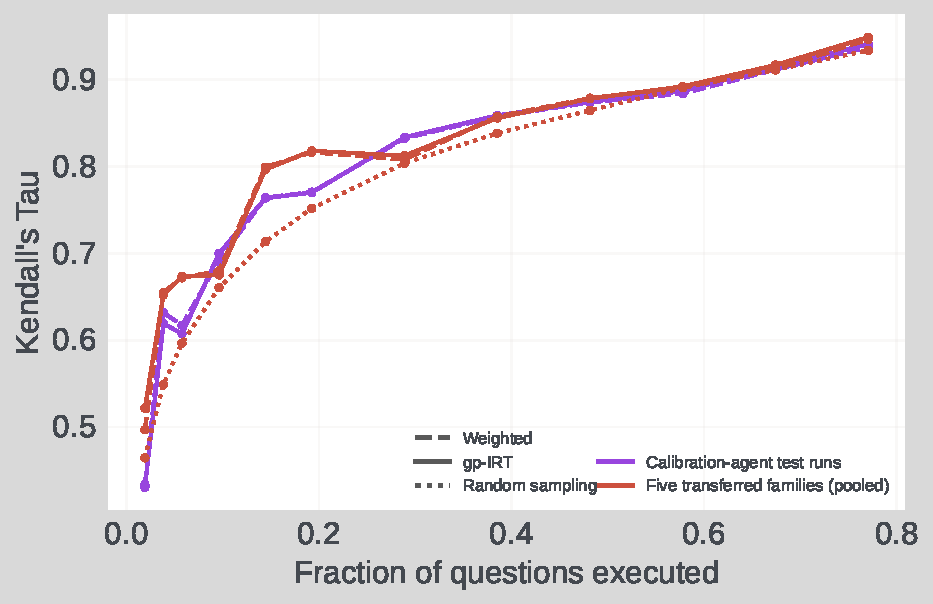
\includegraphics[width=\linewidth]{figures/cross_agent_transfer_kendall.pdf}
        \caption{Kendall's $\tau$.}
        \label{fig:cross-agent-transfer-kendall}
    \end{subfigure}
    \caption{Pooled cross-agent ranking fidelity for a
    difficulty-stratified gp-IRT subset calibrated on the focal family and
    transferred unchanged to 299 runs from five held-out families. Higher
    values are better. Random sampling is averaged over 20 seeds.}
    \label{fig:cross-agent-transfer-ranking}
\end{figure*}

\FloatBarrier

\begin{table*}[t]
  \centering
  \scriptsize
  \setlength{\tabcolsep}{3.5pt}
  \begin{tabular}{rrrrrrr}
    \toprule
    \multicolumn{7}{l}{\textit{(a) Pass-rate MAE (percentage points; lower is better)}} \\
    $k$ & Exec. (\%) & \shortstack{Original\\weighted} & \shortstack{Original\\gp-IRT} & \shortstack{Transfer\\random} & \shortstack{Transfer\\weighted} & \shortstack{Transfer\\gp-IRT} \\
    \midrule
    10 & 1.9 & \underline{8.10} & \textbf{7.57} & 10.96 & \underline{9.83} & \textbf{8.40} \\
    20 & 3.9 & \underline{6.37} & \textbf{5.51} & 7.69 & \underline{6.88} & \textbf{6.15} \\
    30 & 5.8 & \underline{4.63} & \textbf{4.35} & \underline{6.19} & 6.26 & \textbf{5.85} \\
    50 & 9.6 & \underline{3.37} & \textbf{3.28} & 4.67 & \underline{4.18} & \textbf{4.07} \\
    75 & 14.5 & \textbf{3.04} & \underline{3.05} & 3.68 & \underline{3.37} & \textbf{3.32} \\
    100 & 19.3 & \underline{2.71} & \textbf{2.65} & 3.08 & \underline{2.52} & \textbf{2.50} \\
    150 & 28.9 & \underline{2.01} & \textbf{2.00} & 2.29 & \underline{2.25} & \textbf{2.17} \\
    200 & 38.5 & \underline{1.43} & \textbf{1.40} & 1.86 & \underline{1.49} & \textbf{1.47} \\
    250 & 48.2 & \underline{1.17} & \textbf{1.15} & 1.53 & \underline{1.30} & \textbf{1.28} \\
    300 & 57.8 & \underline{1.06} & \textbf{0.99} & 1.24 & \underline{1.21} & \textbf{1.19} \\
    350 & 67.4 & \underline{0.77} & \textbf{0.73} & \textbf{0.99} & 1.05 & \underline{1.02} \\
    400 & 77.1 & \underline{0.51} & \textbf{0.47} & 0.75 & \underline{0.66} & \textbf{0.62} \\
    \midrule
    \multicolumn{7}{l}{\textit{(b) Spearman correlation (higher is better)}} \\
    $k$ & Exec. (\%) & \shortstack{Original\\weighted} & \shortstack{Original\\gp-IRT} & \shortstack{Transfer\\random} & \shortstack{Transfer\\weighted} & \shortstack{Transfer\\gp-IRT} \\
    \midrule
    10 & 1.9 & \underline{0.586} & \textbf{0.598} & 0.600 & \underline{0.648} & \textbf{0.683} \\
    20 & 3.9 & \textbf{0.804} & \underline{0.803} & \underline{0.702} & \textbf{0.817} & \textbf{0.817} \\
    30 & 5.8 & \textbf{0.803} & \underline{0.796} & 0.756 & \underline{0.844} & \textbf{0.847} \\
    50 & 9.6 & \underline{0.876} & \textbf{0.883} & 0.821 & \textbf{0.853} & \underline{0.846} \\
    75 & 14.5 & \textbf{0.924} & \textbf{0.924} & 0.869 & \textbf{0.937} & \underline{0.936} \\
    100 & 19.3 & \textbf{0.930} & \textbf{0.930} & 0.900 & \underline{0.947} & \textbf{0.948} \\
    150 & 28.9 & \underline{0.960} & \textbf{0.961} & 0.935 & \underline{0.938} & \textbf{0.941} \\
    200 & 38.5 & \textbf{0.972} & \textbf{0.972} & \underline{0.955} & \textbf{0.965} & \textbf{0.965} \\
    250 & 48.2 & \underline{0.977} & \textbf{0.978} & \underline{0.968} & \textbf{0.974} & \textbf{0.974} \\
    300 & 57.8 & \underline{0.980} & \textbf{0.981} & \underline{0.979} & \textbf{0.981} & \textbf{0.981} \\
    350 & 67.4 & \underline{0.987} & \textbf{0.988} & 0.986 & \underline{0.987} & \textbf{0.988} \\
    400 & 77.1 & \underline{0.993} & \textbf{0.994} & \underline{0.992} & \textbf{0.995} & \textbf{0.995} \\
    \midrule
    \multicolumn{7}{l}{\textit{(c) Kendall's Tau (higher is better)}} \\
    $k$ & Exec. (\%) & \shortstack{Original\\weighted} & \shortstack{Original\\gp-IRT} & \shortstack{Transfer\\random} & \shortstack{Transfer\\weighted} & \shortstack{Transfer\\gp-IRT} \\
    \midrule
    10 & 1.9 & \textbf{0.434} & \underline{0.431} & 0.465 & \underline{0.497} & \textbf{0.522} \\
    20 & 3.9 & \textbf{0.632} & \underline{0.619} & 0.549 & \textbf{0.655} & \underline{0.652} \\
    30 & 5.8 & \textbf{0.617} & \underline{0.607} & 0.597 & \underline{0.672} & \textbf{0.673} \\
    50 & 9.6 & \underline{0.692} & \textbf{0.700} & 0.661 & \textbf{0.680} & \underline{0.675} \\
    75 & 14.5 & \textbf{0.764} & \textbf{0.764} & 0.713 & \textbf{0.799} & \underline{0.797} \\
    100 & 19.3 & \textbf{0.771} & \underline{0.770} & 0.752 & \underline{0.816} & \textbf{0.818} \\
    150 & 28.9 & \underline{0.832} & \textbf{0.834} & 0.804 & \underline{0.808} & \textbf{0.812} \\
    200 & 38.5 & \underline{0.857} & \textbf{0.859} & 0.838 & \textbf{0.858} & \underline{0.856} \\
    250 & 48.2 & \textbf{0.874} & \textbf{0.874} & 0.865 & \textbf{0.879} & \underline{0.878} \\
    300 & 57.8 & \underline{0.884} & \textbf{0.887} & \underline{0.891} & \underline{0.891} & \textbf{0.892} \\
    350 & 67.4 & \underline{0.912} & \textbf{0.915} & 0.911 & \underline{0.912} & \textbf{0.917} \\
    400 & 77.1 & \underline{0.937} & \textbf{0.941} & 0.934 & \underline{0.946} & \textbf{0.949} \\
    \bottomrule
  \end{tabular}
  \caption{Complete pooled cross-agent transfer results. Original denotes the 287 calibration-agent test runs; Transfer denotes 299 pooled runs from five additional families. Emphasis is computed separately within the original and transferred populations.}
  \label{tab:transfer-pooled-complete}
\end{table*}


\FloatBarrier

\begin{figure*}[t]
    \centering
    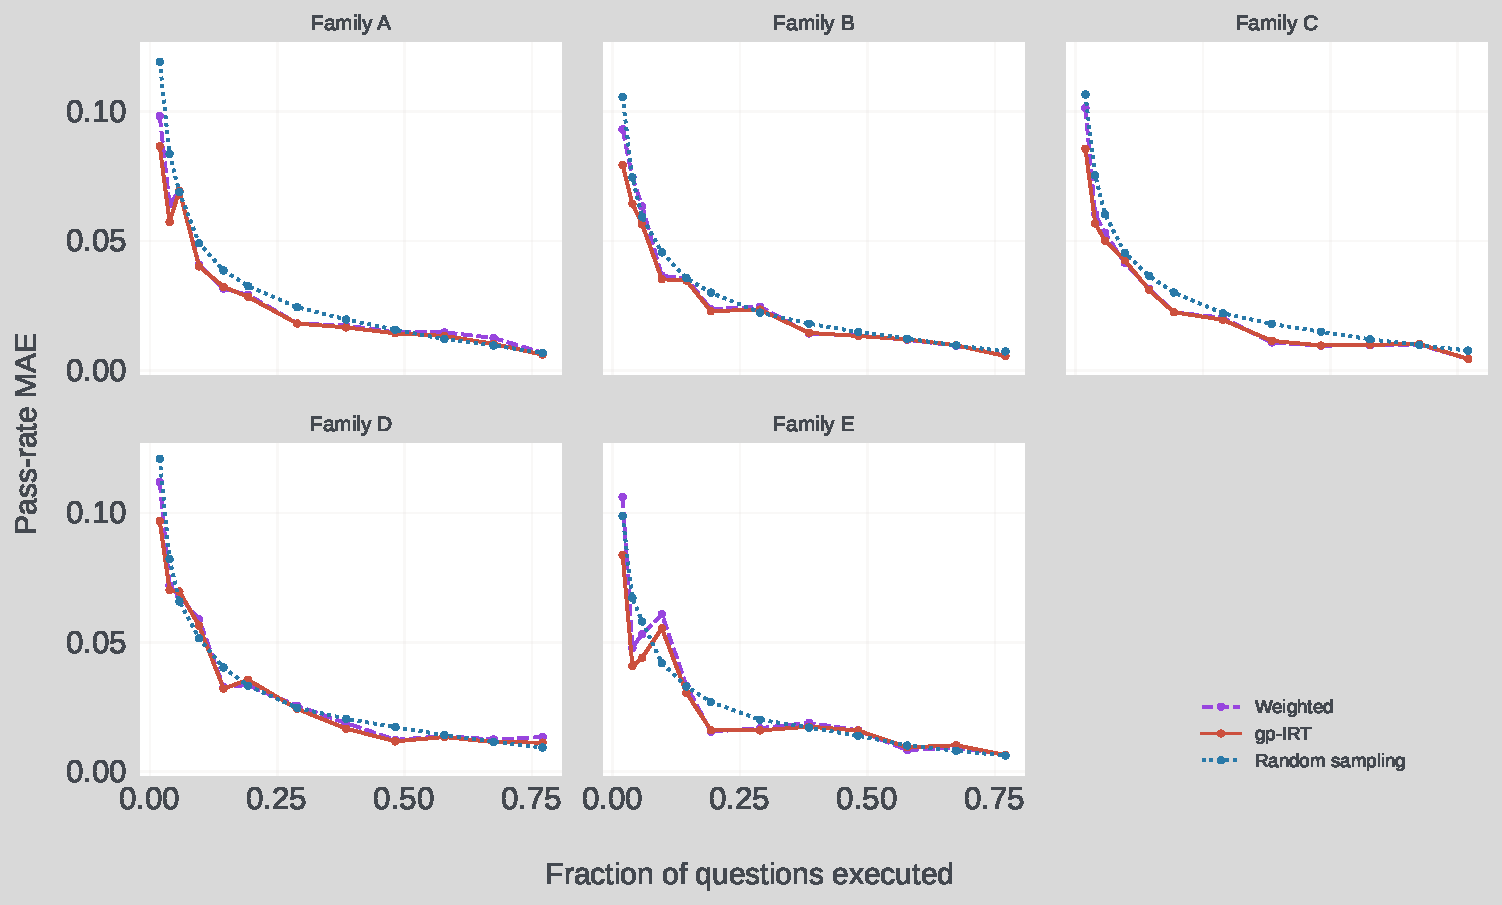
\includegraphics[width=0.82\textwidth]{figures/cross_agent_family_mae_panels.pdf}
    \caption{Cross-agent pass-rate MAE by anonymized family for the transferred
    difficulty-stratified gp-IRT subset and 20-seed random sampling. Lower is
    better. Each panel compares methods on the same held-out runs within that
    family.}
    \label{fig:cross-agent-family-mae}
\end{figure*}

\begin{figure*}[t]
    \centering
    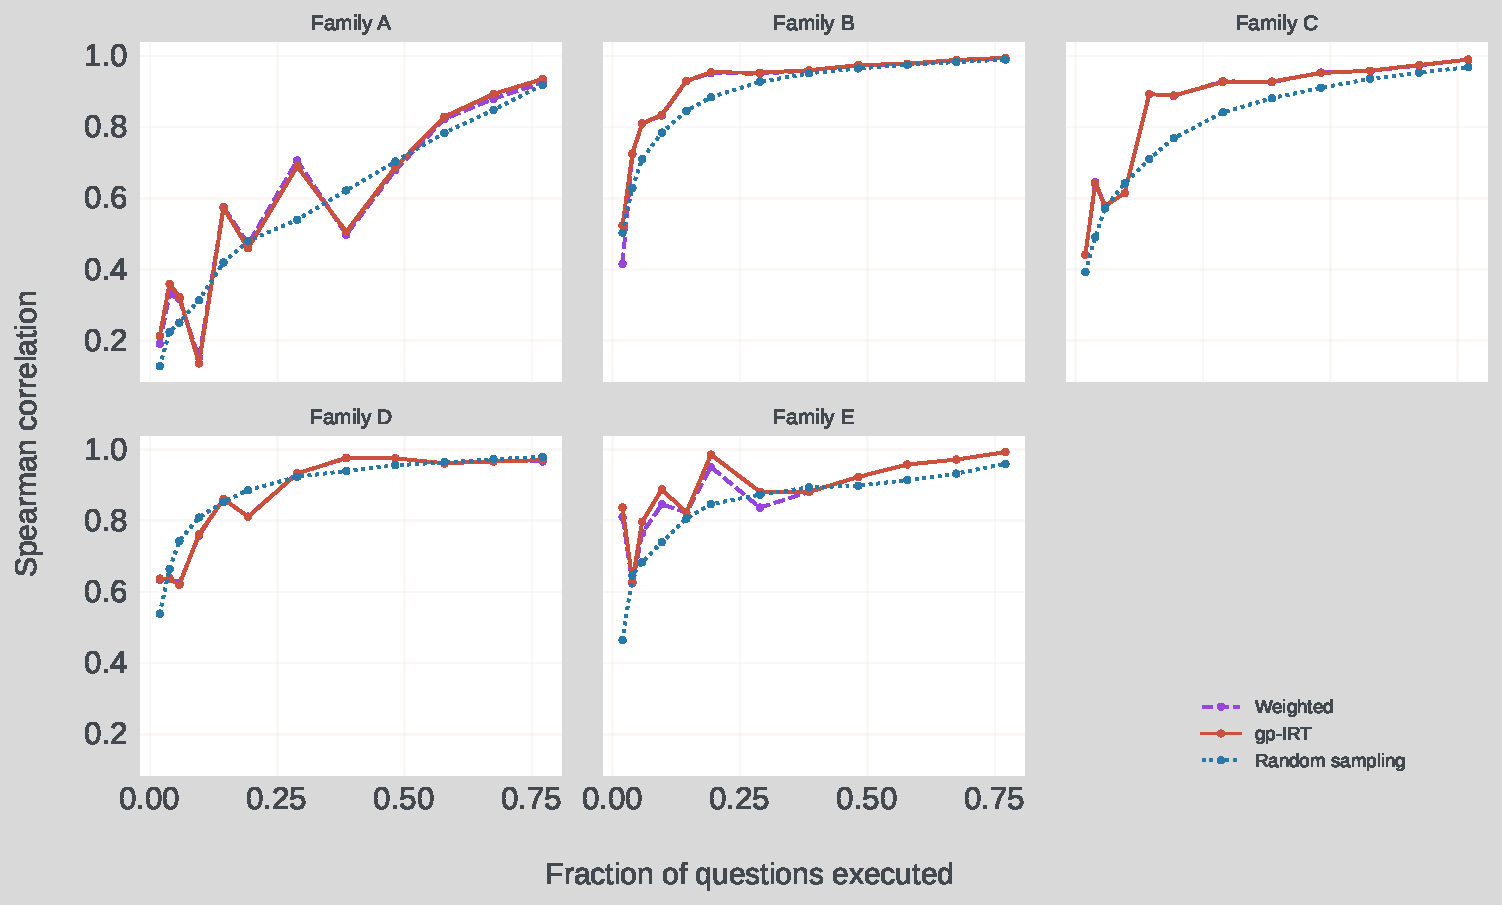
\includegraphics[width=0.82\textwidth]{figures/cross_agent_family_spearman_panels.pdf}
    \caption{Cross-agent Spearman ranking fidelity by anonymized family. Higher
    is better. Correlations are computed within family, and random sampling is
    averaged over 20 seeds.}
    \label{fig:cross-agent-family-spearman}
\end{figure*}

\begin{figure*}[t]
    \centering
    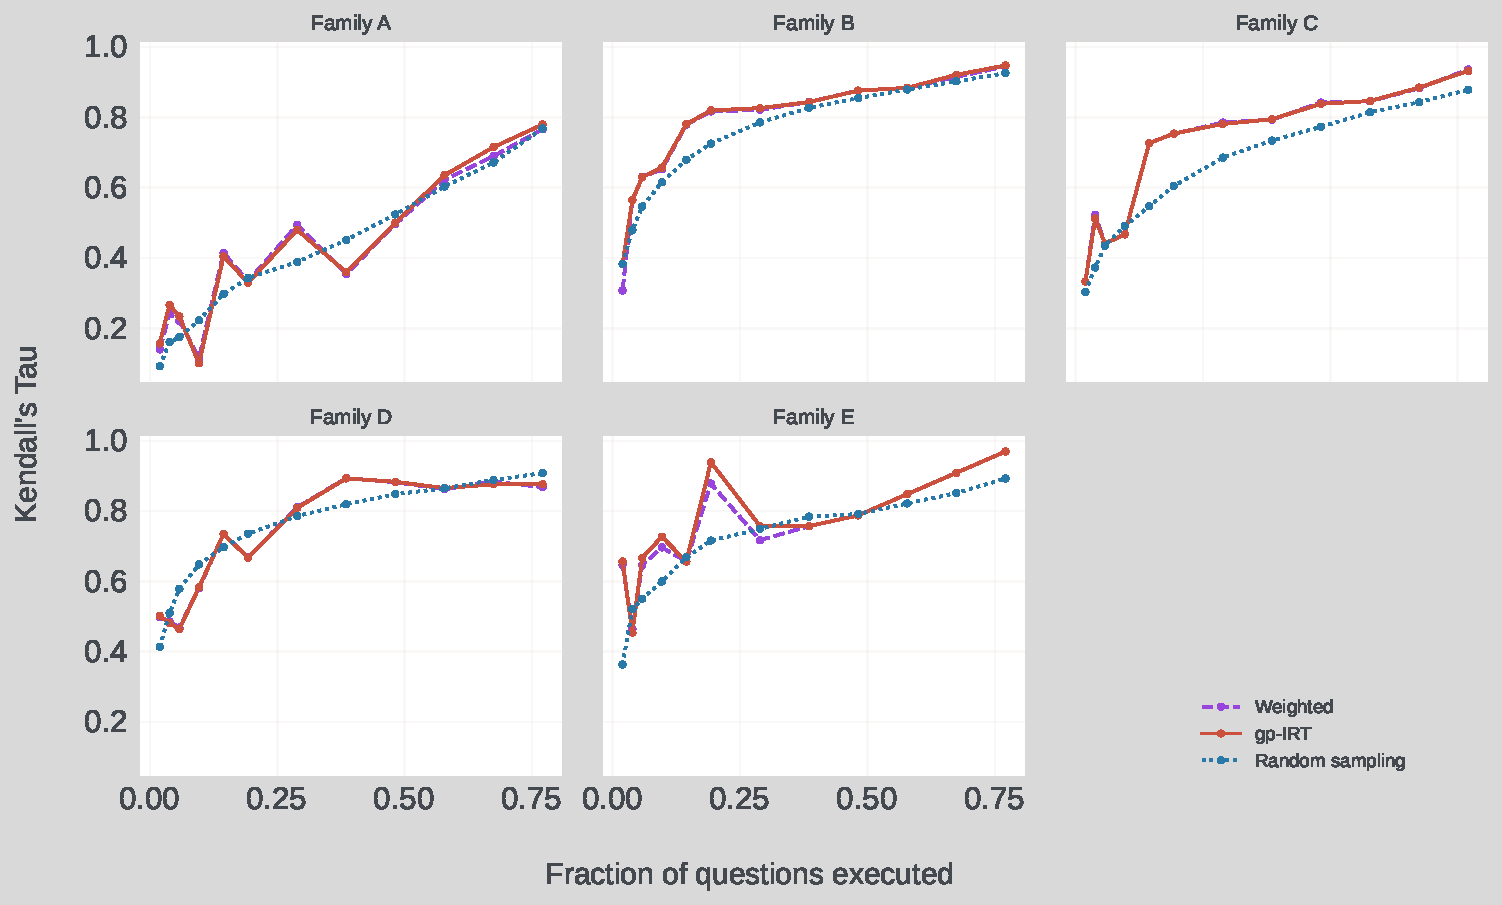
\includegraphics[width=0.82\textwidth]{figures/cross_agent_family_kendall_panels.pdf}
    \caption{Cross-agent Kendall's $\tau$ ranking fidelity by anonymized
    family. Higher is better. Correlations are computed within family, and
    random sampling is averaged over 20 seeds.}
    \label{fig:cross-agent-family-kendall}
\end{figure*}

\FloatBarrier

\begin{table*}[t]
  \centering
  \small
  \setlength{\tabcolsep}{3.5pt}
  \begin{tabular}{rrrrr}
    \toprule
    \multicolumn{5}{l}{\textit{(a) Pass-rate MAE (percentage points; lower is better)}} \\
    $k$ & Exec. (\%) & Random & Weighted & gp-IRT \\
    \midrule
    10 & 1.9 & 11.93 & \underline{9.83} & \textbf{8.66} \\
    20 & 3.9 & 8.37 & \underline{6.42} & \textbf{5.74} \\
    30 & 5.8 & \textbf{6.90} & \underline{6.95} & \underline{6.95} \\
    50 & 9.6 & 4.92 & \underline{4.08} & \textbf{4.02} \\
    75 & 14.5 & 3.86 & \textbf{3.17} & \underline{3.23} \\
    100 & 19.3 & 3.26 & \underline{2.92} & \textbf{2.84} \\
    150 & 28.9 & \underline{2.45} & \textbf{1.82} & \textbf{1.82} \\
    200 & 38.5 & 1.97 & \underline{1.74} & \textbf{1.67} \\
    250 & 48.2 & 1.58 & \underline{1.47} & \textbf{1.44} \\
    300 & 57.8 & \textbf{1.21} & 1.47 & \underline{1.34} \\
    350 & 67.4 & \textbf{0.97} & 1.26 & \underline{1.03} \\
    400 & 77.1 & \underline{0.68} & 0.69 & \textbf{0.61} \\
    \midrule
    \multicolumn{5}{l}{\textit{(b) Spearman correlation (higher is better)}} \\
    $k$ & Exec. (\%) & Random & Weighted & gp-IRT \\
    \midrule
    10 & 1.9 & 0.128 & \underline{0.191} & \textbf{0.213} \\
    20 & 3.9 & 0.223 & \underline{0.330} & \textbf{0.360} \\
    30 & 5.8 & 0.250 & \underline{0.317} & \textbf{0.323} \\
    50 & 9.6 & \textbf{0.314} & \underline{0.151} & 0.136 \\
    75 & 14.5 & 0.419 & \textbf{0.575} & \underline{0.573} \\
    100 & 19.3 & \textbf{0.480} & \underline{0.471} & 0.460 \\
    150 & 28.9 & 0.539 & \textbf{0.706} & \underline{0.689} \\
    200 & 38.5 & \textbf{0.622} & 0.498 & \underline{0.506} \\
    250 & 48.2 & \textbf{0.703} & 0.679 & \underline{0.687} \\
    300 & 57.8 & 0.784 & \underline{0.823} & \textbf{0.829} \\
    350 & 67.4 & 0.848 & \underline{0.879} & \textbf{0.893} \\
    400 & 77.1 & 0.919 & \underline{0.925} & \textbf{0.935} \\
    \midrule
    \multicolumn{5}{l}{\textit{(c) Kendall's Tau (higher is better)}} \\
    $k$ & Exec. (\%) & Random & Weighted & gp-IRT \\
    \midrule
    10 & 1.9 & 0.092 & \underline{0.140} & \textbf{0.157} \\
    20 & 3.9 & 0.161 & \underline{0.241} & \textbf{0.267} \\
    30 & 5.8 & 0.174 & \underline{0.222} & \textbf{0.234} \\
    50 & 9.6 & \textbf{0.223} & \underline{0.115} & 0.100 \\
    75 & 14.5 & 0.298 & \textbf{0.415} & \underline{0.405} \\
    100 & 19.3 & \textbf{0.343} & \underline{0.334} & 0.330 \\
    150 & 28.9 & 0.389 & \textbf{0.494} & \underline{0.480} \\
    200 & 38.5 & \textbf{0.451} & 0.355 & \underline{0.359} \\
    250 & 48.2 & \textbf{0.524} & 0.496 & \underline{0.501} \\
    300 & 57.8 & 0.603 & \underline{0.622} & \textbf{0.636} \\
    350 & 67.4 & 0.672 & \underline{0.690} & \textbf{0.716} \\
    400 & 77.1 & \underline{0.769} & 0.766 & \textbf{0.780} \\
    \bottomrule
  \end{tabular}
  \caption{Complete transfer results for anonymized Family A. Bold and underlining mark the best and second-best displayed values at each budget, respectively.}
  \label{tab:transfer-family-a-complete}
\end{table*}

\begin{table*}[t]
  \centering
  \small
  \setlength{\tabcolsep}{3.5pt}
  \begin{tabular}{rrrrr}
    \toprule
    \multicolumn{5}{l}{\textit{(a) Pass-rate MAE (percentage points; lower is better)}} \\
    $k$ & Exec. (\%) & Random & Weighted & gp-IRT \\
    \midrule
    10 & 1.9 & 10.56 & \underline{9.32} & \textbf{7.94} \\
    20 & 3.9 & \underline{7.46} & \underline{7.46} & \textbf{6.45} \\
    30 & 5.8 & \underline{5.93} & 6.34 & \textbf{5.64} \\
    50 & 9.6 & 4.56 & \underline{3.66} & \textbf{3.53} \\
    75 & 14.5 & 3.57 & \underline{3.56} & \textbf{3.47} \\
    100 & 19.3 & 3.01 & \underline{2.37} & \textbf{2.30} \\
    150 & 28.9 & \textbf{2.24} & 2.47 & \underline{2.35} \\
    200 & 38.5 & 1.81 & \textbf{1.43} & \underline{1.46} \\
    250 & 48.2 & 1.49 & \underline{1.35} & \textbf{1.34} \\
    300 & 57.8 & 1.23 & \textbf{1.19} & \underline{1.20} \\
    350 & 67.4 & \underline{0.97} & \textbf{0.96} & \underline{0.97} \\
    400 & 77.1 & 0.74 & \underline{0.57} & \textbf{0.56} \\
    \midrule
    \multicolumn{5}{l}{\textit{(b) Spearman correlation (higher is better)}} \\
    $k$ & Exec. (\%) & Random & Weighted & gp-IRT \\
    \midrule
    10 & 1.9 & \underline{0.503} & 0.416 & \textbf{0.524} \\
    20 & 3.9 & 0.629 & \underline{0.725} & \textbf{0.726} \\
    30 & 5.8 & \underline{0.710} & \textbf{0.810} & \textbf{0.810} \\
    50 & 9.6 & 0.785 & \underline{0.832} & \textbf{0.835} \\
    75 & 14.5 & 0.845 & \underline{0.929} & \textbf{0.930} \\
    100 & 19.3 & 0.884 & \underline{0.952} & \textbf{0.954} \\
    150 & 28.9 & 0.927 & \underline{0.950} & \textbf{0.953} \\
    200 & 38.5 & 0.951 & \underline{0.959} & \textbf{0.960} \\
    250 & 48.2 & \underline{0.965} & \textbf{0.974} & \textbf{0.974} \\
    300 & 57.8 & 0.975 & \underline{0.977} & \textbf{0.978} \\
    350 & 67.4 & 0.983 & \underline{0.987} & \textbf{0.989} \\
    400 & 77.1 & 0.990 & \underline{0.994} & \textbf{0.995} \\
    \midrule
    \multicolumn{5}{l}{\textit{(c) Kendall's Tau (higher is better)}} \\
    $k$ & Exec. (\%) & Random & Weighted & gp-IRT \\
    \midrule
    10 & 1.9 & \textbf{0.383} & 0.308 & \underline{0.382} \\
    20 & 3.9 & \underline{0.480} & \textbf{0.565} & \textbf{0.565} \\
    30 & 5.8 & 0.546 & \textbf{0.631} & \underline{0.630} \\
    50 & 9.6 & 0.615 & \underline{0.652} & \textbf{0.657} \\
    75 & 14.5 & 0.680 & \underline{0.780} & \textbf{0.781} \\
    100 & 19.3 & 0.726 & \underline{0.817} & \textbf{0.820} \\
    150 & 28.9 & 0.786 & \underline{0.821} & \textbf{0.827} \\
    200 & 38.5 & \underline{0.827} & \textbf{0.844} & \textbf{0.844} \\
    250 & 48.2 & 0.855 & \textbf{0.877} & \underline{0.876} \\
    300 & 57.8 & \underline{0.879} & \textbf{0.884} & \textbf{0.884} \\
    350 & 67.4 & 0.903 & \underline{0.915} & \textbf{0.921} \\
    400 & 77.1 & 0.926 & \underline{0.945} & \textbf{0.948} \\
    \bottomrule
  \end{tabular}
  \caption{Complete transfer results for anonymized Family B. Bold and underlining mark the best and second-best displayed values at each budget, respectively.}
  \label{tab:transfer-family-b-complete}
\end{table*}

\begin{table*}[t]
  \centering
  \small
  \setlength{\tabcolsep}{3.5pt}
  \begin{tabular}{rrrrr}
    \toprule
    \multicolumn{5}{l}{\textit{(a) Pass-rate MAE (percentage points; lower is better)}} \\
    $k$ & Exec. (\%) & Random & Weighted & gp-IRT \\
    \midrule
    10 & 1.9 & 10.66 & \underline{10.14} & \textbf{8.57} \\
    20 & 3.9 & 7.54 & \underline{6.03} & \textbf{5.68} \\
    30 & 5.8 & 6.04 & \underline{5.31} & \textbf{5.01} \\
    50 & 9.6 & 4.55 & \textbf{4.16} & \underline{4.26} \\
    75 & 14.5 & 3.65 & \underline{3.16} & \textbf{3.11} \\
    100 & 19.3 & \underline{3.01} & \textbf{2.25} & \textbf{2.25} \\
    150 & 28.9 & 2.21 & \underline{2.04} & \textbf{1.96} \\
    200 & 38.5 & 1.80 & \textbf{1.09} & \underline{1.15} \\
    250 & 48.2 & 1.50 & \textbf{0.96} & \underline{0.97} \\
    300 & 57.8 & 1.21 & \textbf{0.97} & \underline{0.99} \\
    350 & 67.4 & \textbf{0.98} & \underline{1.00} & 1.03 \\
    400 & 77.1 & \underline{0.77} & \textbf{0.45} & \textbf{0.45} \\
    \midrule
    \multicolumn{5}{l}{\textit{(b) Spearman correlation (higher is better)}} \\
    $k$ & Exec. (\%) & Random & Weighted & gp-IRT \\
    \midrule
    10 & 1.9 & \underline{0.393} & \textbf{0.441} & \textbf{0.441} \\
    20 & 3.9 & 0.491 & \textbf{0.645} & \underline{0.641} \\
    30 & 5.8 & \underline{0.572} & \textbf{0.579} & \textbf{0.579} \\
    50 & 9.6 & \textbf{0.642} & \underline{0.614} & \underline{0.614} \\
    75 & 14.5 & \underline{0.711} & \textbf{0.893} & \textbf{0.893} \\
    100 & 19.3 & 0.768 & \underline{0.888} & \textbf{0.889} \\
    150 & 28.9 & 0.841 & \textbf{0.929} & \underline{0.927} \\
    200 & 38.5 & 0.881 & \underline{0.926} & \textbf{0.928} \\
    250 & 48.2 & 0.910 & \textbf{0.953} & \underline{0.952} \\
    300 & 57.8 & 0.936 & \underline{0.958} & \textbf{0.959} \\
    350 & 67.4 & 0.953 & \underline{0.973} & \textbf{0.974} \\
    400 & 77.1 & \underline{0.969} & \textbf{0.990} & \textbf{0.990} \\
    \midrule
    \multicolumn{5}{l}{\textit{(c) Kendall's Tau (higher is better)}} \\
    $k$ & Exec. (\%) & Random & Weighted & gp-IRT \\
    \midrule
    10 & 1.9 & \underline{0.303} & \textbf{0.333} & \textbf{0.333} \\
    20 & 3.9 & 0.373 & \textbf{0.523} & \underline{0.513} \\
    30 & 5.8 & \underline{0.435} & \textbf{0.441} & \textbf{0.441} \\
    50 & 9.6 & \textbf{0.491} & \underline{0.467} & \underline{0.467} \\
    75 & 14.5 & \underline{0.548} & \textbf{0.727} & \textbf{0.727} \\
    100 & 19.3 & \underline{0.605} & \textbf{0.754} & \textbf{0.754} \\
    150 & 28.9 & 0.686 & \textbf{0.786} & \underline{0.781} \\
    200 & 38.5 & 0.734 & \underline{0.794} & \textbf{0.795} \\
    250 & 48.2 & 0.773 & \textbf{0.843} & \underline{0.839} \\
    300 & 57.8 & 0.815 & \underline{0.846} & \textbf{0.847} \\
    350 & 67.4 & 0.843 & \underline{0.884} & \textbf{0.885} \\
    400 & 77.1 & 0.879 & \textbf{0.936} & \underline{0.933} \\
    \bottomrule
  \end{tabular}
  \caption{Complete transfer results for anonymized Family C. Bold and underlining mark the best and second-best displayed values at each budget, respectively.}
  \label{tab:transfer-family-c-complete}
\end{table*}

\begin{table*}[t]
  \centering
  \small
  \setlength{\tabcolsep}{3.5pt}
  \begin{tabular}{rrrrr}
    \toprule
    \multicolumn{5}{l}{\textit{(a) Pass-rate MAE (percentage points; lower is better)}} \\
    $k$ & Exec. (\%) & Random & Weighted & gp-IRT \\
    \midrule
    10 & 1.9 & 12.09 & \underline{11.20} & \textbf{9.69} \\
    20 & 3.9 & 8.21 & \underline{7.20} & \textbf{7.01} \\
    30 & 5.8 & \textbf{6.58} & \underline{6.79} & 6.96 \\
    50 & 9.6 & \textbf{5.16} & 5.89 & \underline{5.65} \\
    75 & 14.5 & 4.03 & \underline{3.27} & \textbf{3.21} \\
    100 & 19.3 & \textbf{3.32} & \underline{3.35} & 3.55 \\
    150 & 28.9 & \underline{2.47} & 2.54 & \textbf{2.43} \\
    200 & 38.5 & 2.05 & \underline{1.88} & \textbf{1.67} \\
    250 & 48.2 & 1.72 & \underline{1.24} & \textbf{1.18} \\
    300 & 57.8 & 1.42 & \underline{1.38} & \textbf{1.34} \\
    350 & 67.4 & \underline{1.16} & 1.25 & \textbf{1.15} \\
    400 & 77.1 & \textbf{0.94} & 1.34 & \underline{1.13} \\
    \midrule
    \multicolumn{5}{l}{\textit{(b) Spearman correlation (higher is better)}} \\
    $k$ & Exec. (\%) & Random & Weighted & gp-IRT \\
    \midrule
    10 & 1.9 & 0.539 & \underline{0.634} & \textbf{0.638} \\
    20 & 3.9 & \textbf{0.664} & \underline{0.639} & 0.636 \\
    30 & 5.8 & \textbf{0.744} & \underline{0.625} & 0.620 \\
    50 & 9.6 & \textbf{0.809} & 0.758 & \underline{0.762} \\
    75 & 14.5 & \underline{0.853} & \textbf{0.861} & \textbf{0.861} \\
    100 & 19.3 & \textbf{0.886} & \underline{0.812} & 0.811 \\
    150 & 28.9 & \underline{0.924} & \textbf{0.933} & \textbf{0.933} \\
    200 & 38.5 & 0.940 & \underline{0.976} & \textbf{0.977} \\
    250 & 48.2 & 0.956 & \underline{0.975} & \textbf{0.976} \\
    300 & 57.8 & \textbf{0.964} & 0.961 & \underline{0.962} \\
    350 & 67.4 & \textbf{0.973} & \underline{0.969} & 0.967 \\
    400 & 77.1 & \textbf{0.980} & 0.967 & \underline{0.970} \\
    \midrule
    \multicolumn{5}{l}{\textit{(c) Kendall's Tau (higher is better)}} \\
    $k$ & Exec. (\%) & Random & Weighted & gp-IRT \\
    \midrule
    10 & 1.9 & 0.414 & \underline{0.499} & \textbf{0.502} \\
    20 & 3.9 & \textbf{0.510} & \underline{0.486} & 0.481 \\
    30 & 5.8 & \textbf{0.580} & \underline{0.469} & 0.464 \\
    50 & 9.6 & \textbf{0.649} & 0.581 & \underline{0.583} \\
    75 & 14.5 & \underline{0.697} & \textbf{0.735} & \textbf{0.735} \\
    100 & 19.3 & \textbf{0.736} & \underline{0.668} & 0.667 \\
    150 & 28.9 & 0.786 & \textbf{0.811} & \underline{0.809} \\
    200 & 38.5 & 0.820 & \textbf{0.894} & \underline{0.893} \\
    250 & 48.2 & 0.848 & \underline{0.883} & \textbf{0.884} \\
    300 & 57.8 & \underline{0.865} & 0.862 & \textbf{0.866} \\
    350 & 67.4 & \textbf{0.889} & \underline{0.884} & 0.876 \\
    400 & 77.1 & \textbf{0.909} & 0.868 & \underline{0.876} \\
    \bottomrule
  \end{tabular}
  \caption{Complete transfer results for anonymized Family D. Bold and underlining mark the best and second-best displayed values at each budget, respectively.}
  \label{tab:transfer-family-d-complete}
\end{table*}

\begin{table*}[t]
  \centering
  \small
  \setlength{\tabcolsep}{3.5pt}
  \begin{tabular}{rrrrr}
    \toprule
    \multicolumn{5}{l}{\textit{(a) Pass-rate MAE (percentage points; lower is better)}} \\
    $k$ & Exec. (\%) & Random & Weighted & gp-IRT \\
    \midrule
    10 & 1.9 & \underline{9.88} & 10.61 & \textbf{8.38} \\
    20 & 3.9 & 6.72 & \underline{4.79} & \textbf{4.09} \\
    30 & 5.8 & 5.80 & \underline{5.33} & \textbf{4.40} \\
    50 & 9.6 & \textbf{4.20} & 6.09 & \underline{5.54} \\
    75 & 14.5 & \underline{3.30} & 3.32 & \textbf{3.05} \\
    100 & 19.3 & 2.70 & \textbf{1.55} & \underline{1.61} \\
    150 & 28.9 & 2.01 & \underline{1.69} & \textbf{1.60} \\
    200 & 38.5 & \textbf{1.71} & 1.89 & \underline{1.74} \\
    250 & 48.2 & \textbf{1.40} & 1.60 & \underline{1.59} \\
    300 & 57.8 & 1.02 & \textbf{0.84} & \underline{0.94} \\
    350 & 67.4 & \textbf{0.81} & \underline{0.94} & 1.03 \\
    400 & 77.1 & \textbf{0.62} & 0.66 & \underline{0.65} \\
    \midrule
    \multicolumn{5}{l}{\textit{(b) Spearman correlation (higher is better)}} \\
    $k$ & Exec. (\%) & Random & Weighted & gp-IRT \\
    \midrule
    10 & 1.9 & 0.464 & \underline{0.810} & \textbf{0.837} \\
    20 & 3.9 & \textbf{0.646} & 0.624 & \underline{0.629} \\
    30 & 5.8 & 0.684 & \underline{0.765} & \textbf{0.797} \\
    50 & 9.6 & 0.740 & \underline{0.846} & \textbf{0.888} \\
    75 & 14.5 & \underline{0.806} & \textbf{0.823} & \textbf{0.823} \\
    100 & 19.3 & 0.847 & \underline{0.951} & \textbf{0.986} \\
    150 & 28.9 & \underline{0.873} & 0.837 & \textbf{0.881} \\
    200 & 38.5 & \textbf{0.894} & \underline{0.881} & \underline{0.881} \\
    250 & 48.2 & \underline{0.898} & \textbf{0.923} & \textbf{0.923} \\
    300 & 57.8 & \underline{0.914} & \textbf{0.958} & \textbf{0.958} \\
    350 & 67.4 & \underline{0.933} & \textbf{0.972} & \textbf{0.972} \\
    400 & 77.1 & \underline{0.960} & \textbf{0.993} & \textbf{0.993} \\
    \midrule
    \multicolumn{5}{l}{\textit{(c) Kendall's Tau (higher is better)}} \\
    $k$ & Exec. (\%) & Random & Weighted & gp-IRT \\
    \midrule
    10 & 1.9 & 0.364 & \underline{0.647} & \textbf{0.657} \\
    20 & 3.9 & \textbf{0.522} & \underline{0.465} & 0.455 \\
    30 & 5.8 & 0.551 & \underline{0.646} & \textbf{0.667} \\
    50 & 9.6 & 0.600 & \underline{0.697} & \textbf{0.727} \\
    75 & 14.5 & \textbf{0.669} & \underline{0.657} & \underline{0.657} \\
    100 & 19.3 & 0.716 & \underline{0.879} & \textbf{0.939} \\
    150 & 28.9 & \underline{0.749} & 0.718 & \textbf{0.758} \\
    200 & 38.5 & \textbf{0.785} & \underline{0.758} & \underline{0.758} \\
    250 & 48.2 & \textbf{0.792} & \underline{0.788} & \underline{0.788} \\
    300 & 57.8 & \underline{0.822} & \textbf{0.848} & \textbf{0.848} \\
    350 & 67.4 & \underline{0.852} & \textbf{0.909} & \textbf{0.909} \\
    400 & 77.1 & \underline{0.893} & \textbf{0.970} & \textbf{0.970} \\
    \bottomrule
  \end{tabular}
  \caption{Complete transfer results for anonymized Family E. Bold and underlining mark the best and second-best displayed values at each budget, respectively.}
  \label{tab:transfer-family-e-complete}
\end{table*}


\FloatBarrier

\begin{figure*}[t]
    \centering
    \begin{subfigure}[t]{0.49\textwidth}
        \centering
        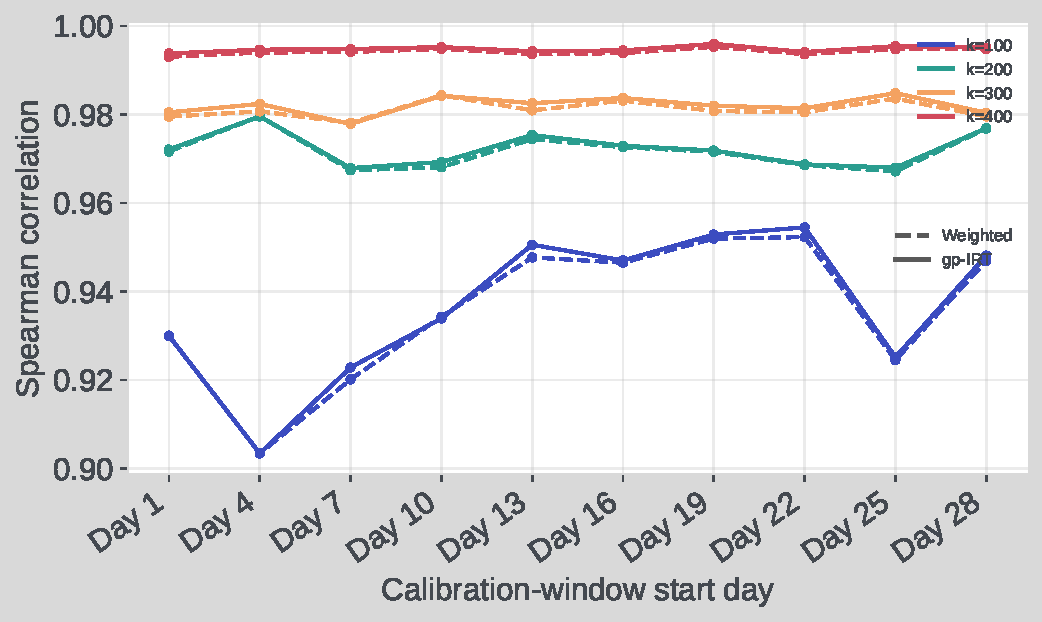
\includegraphics[width=\linewidth]{figures/calibration_window_spearman.pdf}
        \caption{Spearman correlation.}
        \label{fig:calibration-window-spearman}
    \end{subfigure}
    \hfill
    \begin{subfigure}[t]{0.49\textwidth}
        \centering
        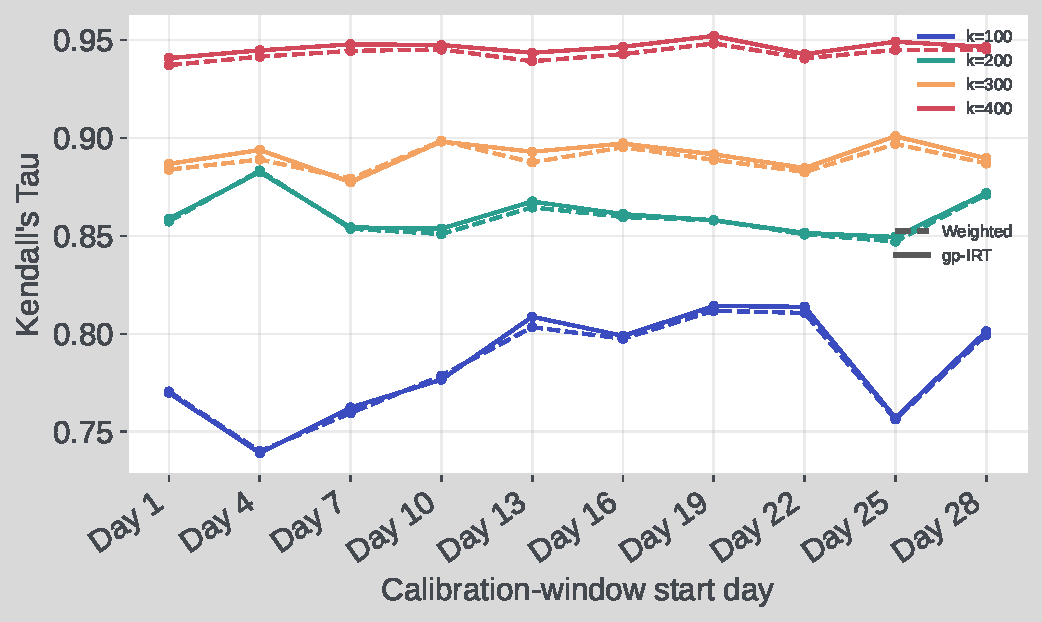
\includegraphics[width=\linewidth]{figures/calibration_window_kendall.pdf}
        \caption{Kendall's $\tau$.}
        \label{fig:calibration-window-kendall}
    \end{subfigure}
    \caption{Ranking-fidelity sensitivity of difficulty-stratified fixed
    subsets to nested calibration windows ending Day 28. Higher values are
    better. Windows vary jointly in historical range and calibration-run
    count; all curves use the same 287 held-out evaluation runs.}
    \label{fig:calibration-window-ranking}
\end{figure*}

\FloatBarrier

\begin{table*}[t]
  \centering
  \scriptsize
  \setlength{\tabcolsep}{2.8pt}
  \begin{tabular}{lrrrrrrrrr}
    \toprule
    \multicolumn{10}{l}{\textit{(a) Pass-rate MAE (percentage points; lower is better)}} \\
    \multicolumn{2}{c}{} & \multicolumn{2}{c}{${k=100}$} & \multicolumn{2}{c}{${k=200}$} & \multicolumn{2}{c}{${k=300}$} & \multicolumn{2}{c}{${k=400}$} \\
    Start & Runs & Weighted & gp-IRT & Weighted & gp-IRT & Weighted & gp-IRT & Weighted & gp-IRT \\
    \midrule
    Day 1 & 287 & 2.71 & 2.65 & 1.43 & 1.40 & 1.06 & 0.99 & 0.51 & 0.47 \\
    Day 4 & 258 & 2.86 & 2.97 & 1.42 & 1.35 & 1.14 & 1.06 & 0.53 & 0.52 \\
    Day 7 & 222 & 2.71 & 2.69 & 1.50 & 1.49 & 1.29 & 1.35 & 0.50 & 0.45 \\
    Day 10 & 192 & 2.39 & 2.36 & 1.66 & 1.59 & 0.97 & 0.98 & 0.52 & 0.52 \\
    Day 13 & 157 & 2.12 & 2.04 & 1.43 & 1.35 & 1.16 & 1.05 & 0.55 & 0.52 \\
    Day 16 & 128 & 2.33 & 2.30 & 1.49 & 1.45 & 0.95 & 0.93 & 0.51 & 0.50 \\
    Day 19 & 101 & 2.14 & 2.15 & 1.59 & 1.59 & 0.97 & 0.94 & 0.49 & 0.43 \\
    Day 22 & 74 & 2.06 & 2.04 & 1.46 & 1.49 & 1.12 & 1.14 & 0.58 & 0.56 \\
    Day 25 & 43 & 2.54 & 2.46 & 1.60 & 1.58 & 1.22 & 1.14 & 0.58 & 0.52 \\
    Day 28 & 14 & 2.20 & 2.19 & 1.45 & 1.41 & 1.04 & 1.03 & 0.51 & 0.51 \\
    \midrule
    \multicolumn{10}{l}{\textit{(b) Spearman correlation (higher is better)}} \\
    \multicolumn{2}{c}{} & \multicolumn{2}{c}{${k=100}$} & \multicolumn{2}{c}{${k=200}$} & \multicolumn{2}{c}{${k=300}$} & \multicolumn{2}{c}{${k=400}$} \\
    Start & Runs & Weighted & gp-IRT & Weighted & gp-IRT & Weighted & gp-IRT & Weighted & gp-IRT \\
    \midrule
    Day 1 & 287 & 0.930 & 0.930 & 0.972 & 0.972 & 0.980 & 0.981 & 0.993 & 0.994 \\
    Day 4 & 258 & 0.903 & 0.903 & 0.980 & 0.980 & 0.981 & 0.982 & 0.994 & 0.995 \\
    Day 7 & 222 & 0.920 & 0.923 & 0.967 & 0.968 & 0.978 & 0.978 & 0.994 & 0.995 \\
    Day 10 & 192 & 0.934 & 0.934 & 0.968 & 0.969 & 0.984 & 0.984 & 0.995 & 0.995 \\
    Day 13 & 157 & 0.948 & 0.951 & 0.974 & 0.975 & 0.981 & 0.983 & 0.994 & 0.994 \\
    Day 16 & 128 & 0.947 & 0.947 & 0.973 & 0.973 & 0.983 & 0.984 & 0.994 & 0.994 \\
    Day 19 & 101 & 0.952 & 0.953 & 0.972 & 0.972 & 0.981 & 0.982 & 0.995 & 0.996 \\
    Day 22 & 74 & 0.952 & 0.955 & 0.969 & 0.969 & 0.981 & 0.981 & 0.994 & 0.994 \\
    Day 25 & 43 & 0.925 & 0.925 & 0.967 & 0.968 & 0.984 & 0.985 & 0.995 & 0.995 \\
    Day 28 & 14 & 0.947 & 0.948 & 0.977 & 0.977 & 0.980 & 0.980 & 0.995 & 0.995 \\
    \midrule
    \multicolumn{10}{l}{\textit{(c) Kendall's Tau (higher is better)}} \\
    \multicolumn{2}{c}{} & \multicolumn{2}{c}{${k=100}$} & \multicolumn{2}{c}{${k=200}$} & \multicolumn{2}{c}{${k=300}$} & \multicolumn{2}{c}{${k=400}$} \\
    Start & Runs & Weighted & gp-IRT & Weighted & gp-IRT & Weighted & gp-IRT & Weighted & gp-IRT \\
    \midrule
    Day 1 & 287 & 0.771 & 0.770 & 0.857 & 0.859 & 0.884 & 0.887 & 0.937 & 0.941 \\
    Day 4 & 258 & 0.740 & 0.739 & 0.883 & 0.883 & 0.889 & 0.894 & 0.942 & 0.945 \\
    Day 7 & 222 & 0.760 & 0.762 & 0.854 & 0.854 & 0.879 & 0.877 & 0.944 & 0.948 \\
    Day 10 & 192 & 0.779 & 0.777 & 0.851 & 0.854 & 0.899 & 0.898 & 0.945 & 0.947 \\
    Day 13 & 157 & 0.803 & 0.809 & 0.865 & 0.868 & 0.888 & 0.893 & 0.939 & 0.944 \\
    Day 16 & 128 & 0.798 & 0.799 & 0.860 & 0.861 & 0.895 & 0.897 & 0.943 & 0.947 \\
    Day 19 & 101 & 0.812 & 0.814 & 0.858 & 0.858 & 0.889 & 0.892 & 0.948 & 0.952 \\
    Day 22 & 74 & 0.811 & 0.814 & 0.851 & 0.852 & 0.883 & 0.885 & 0.941 & 0.943 \\
    Day 25 & 43 & 0.756 & 0.757 & 0.847 & 0.849 & 0.897 & 0.901 & 0.945 & 0.949 \\
    Day 28 & 14 & 0.799 & 0.801 & 0.871 & 0.872 & 0.887 & 0.890 & 0.945 & 0.947 \\
    \bottomrule
  \end{tabular}
  \caption{Complete calibration-window sensitivity results. All windows end Day 28 and use the same 287 held-out runs. MAE is in percentage points. Values are not emphasized because the windows form a sensitivity sweep rather than prespecified competing methods.}
  \label{tab:calibration-window-complete}
\end{table*}


\FloatBarrier
